\documentclass{article}
\usepackage{tikz}
\usetikzlibrary{mindmap, shapes.geometric}

\title{TikZ Mindmap Example with Branch Lines}
\author{}
\date{}

\begin{document}
\maketitle

\section*{Ccomplexity and Neuroscience mindmap}

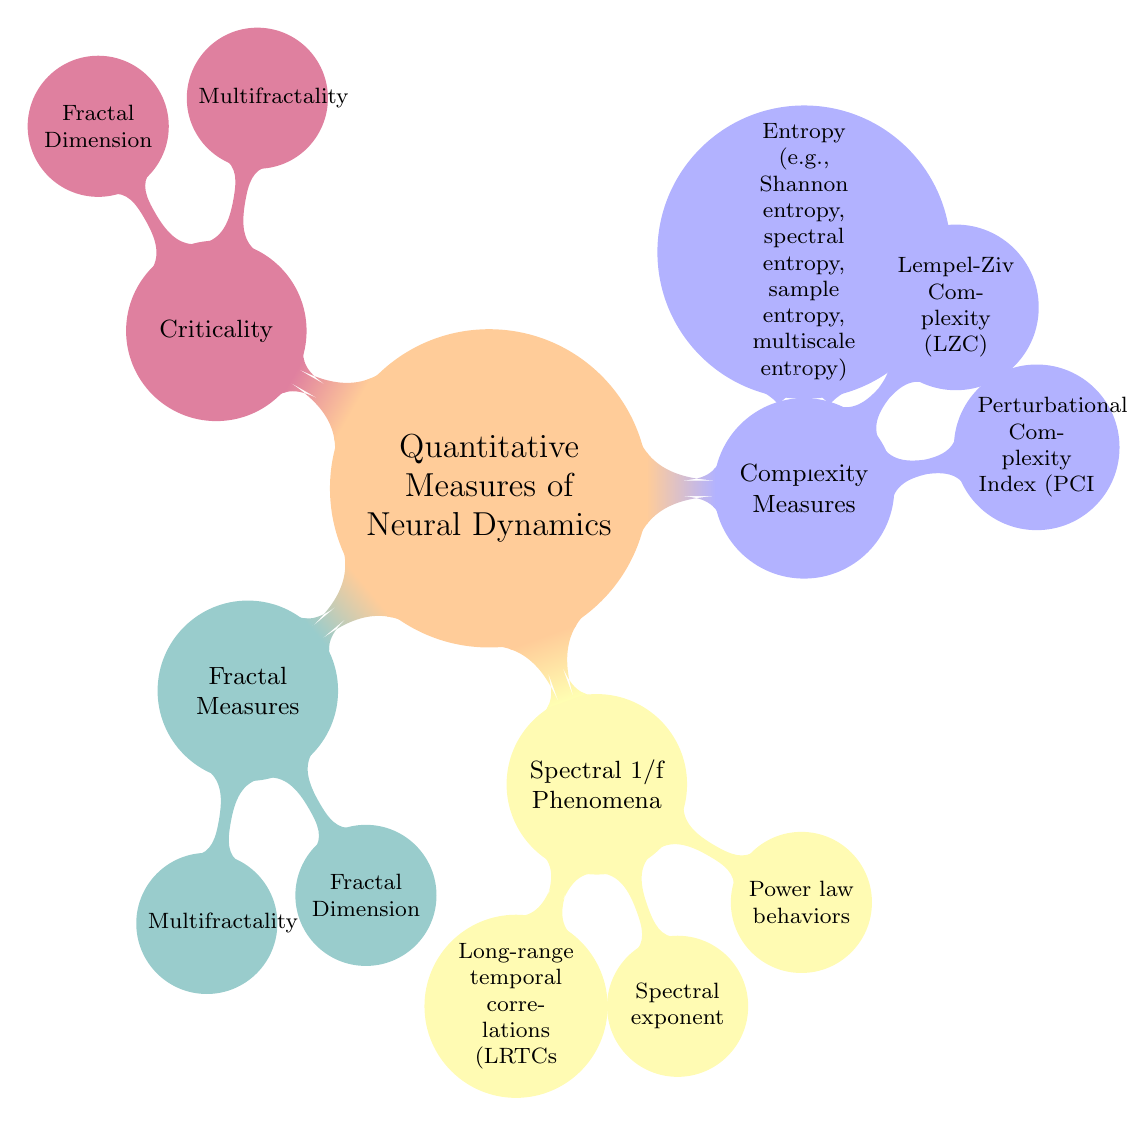
\begin{tikzpicture}[mindmap, grow cyclic, every node/.style=concept, concept color=orange!40,
    level 1/.append style={level distance=4cm,sibling angle=70},
    level 2/.append style={level distance=3cm,sibling angle=40},
    text=black]
  \node[concept, concept color=orange!40, text=black] {Quantitative Measures of Neural Dynamics}
    [clockwise from=0]
    child[concept color=blue!30] {
      node[concept] {Complexity Measures}
      [clockwise from=90]
      child { node[concept] {Entropy (e.g., Shannon entropy, spectral entropy, sample entropy, multiscale entropy)} }
      child { node[concept] {Lempel-Ziv Complexity (LZC)} }
      child { node[concept] {Perturbational Complexity Index (PCI} }
    }
    child[concept color=yellow!30] {
      node[concept] {Spectral 1/f Phenomena }
      [clockwise from=-30]
      child { node[concept] {Power law behaviors} }
      child { node[concept] {Spectral exponent} }      
      child { node[concept] {Long-range temporal correlations (LRTCs} }
    }
    child[concept color=teal!40] { node[concept] {Fractal Measures}
    [clockwise from=-60]
    child { node[concept] {Fractal Dimension} }
    child { node[concept] {Multifractality} } }
    child[concept color=purple!50] { node[concept] { Criticality}
     [clockwise from=120]
    child { node[concept] {Fractal Dimension} }
    child { node[concept] {Multifractality} }};
    
\end{tikzpicture}

\end{document}